\chapter{Background \& Related Work}
\label{chap:background}

In this section, constraint optimization and the distributed, as well as dynamic variants are briefly explained and brought into context of the related work. Also, the meeting scheduling problem is described and different algorithm designs and their advantages and disadvantages are explained and related work is mentioned.
    
\section{Dynamic Distributed Constraint Optimization}

% -----------------Constraint Optimization --------------------
    
A constraint optimization problem contains of a set of variables \(V=\{V_{1},V_{2}, ...,  V_{n}\}\). These variables are assigned to a value or state \(s_{j} \in S_{j}\), which is contained in a set of possible values defined by a finite problem domain \(D=\{D_{1},D_{2}, ...,  D_{n}\}\). A constraint \(C = <V_{c}, R_{c}>\) contains one (unary), two (binary) or multiple (k-ary) variables and their relationship. The constraint defines a rule for the variables that needs to be fulfilled. One of those rules could be that none of the variables should take the same value. This would for example be the case for a meeting scheduling problem where none of the meetings should take place at the same time. \newline
A utility function \(u_{{c}_{k}}(S_{{c}_{k}})\) needs to be formulated that defines a certain cost respectively reward for a given configuration of the involved states. The global utility function \(u_{g}\) would then be the summation of all utility functions of all constraints. 

\[u_{g}(s) = u_{c_{1}}(s_{c_{1}}) \oplus \cdots \oplus u_{c_{k}}(s_{c_{k}}) \oplus \cdots \oplus u_{c_{l}}(s_{c_{l}}) \] 

Constraints can be attributed with varying levels of importance through weighting. One can, instead of so-called soft constraints, define hard constraints by multiplying their utility instead of using addition in the global utility function. By defining the utility of a violated hard constraint as 0, the global utility would also go to 0 if this hard constraint is not satisfied \cite{Chapman2011, Petcu2003}. A problem only containing hard constraints would represent a constraint satisfaction problem.

\[ u_{g}(s) = \prod_{\substack{hc_{k} \in HC}} u_{SC_{g}}(s) \bigg( \sum_{sc_{k} \in SC} u_{SC_{g}}(s) \bigg)\] 


% ----------------- Distributed Constraint Optimization --------------------
The definition of a distributed constraint problem extends the basic constraint optimization by distributing sets of variables to autonomous agents. These agents all have the goal to maximize the utility of their variables in a private utility function and thereby also contribute to a global utility function. Agents whose variables are linked to a common constraint are called neighbours \cite{Chapman2011, Farinelli, Petcu2003}.
\newline\newline 
% ----------------- Dynamic Distributed Constraint Optimization --------------------
As a further extension to the optimization, the problem definition is moved from a static to a dynamic attribute. Constraints can change and  therefore change neighbourhoods and the outcome of private and global utility functions. A change of constraints inherently changes the area of satisfying solutions if hard constraints have been included in a problem definition. Nguyen et al. state that changing the constraints might lead to the discovery of a better global optima.\cite{Nguyen2012}. Mailler et al. define a dynamic DCSP as a sequence of DCSPs \(\{P_{0}, P_{1}, ..., P_{n}\}\) where every DCSP is a static problem definition. \(P_{i}\) is therfore a result of the previous DSCP in the sequence and the added and removed constraints: \(P_{i} = P_{i-1} + c_{i^{a}} - c_{i^{r}}\) \cite{Maillera}. This definition should also hold for DCOPs. Utility functions could also be dynamically changed. Modifying this property could especially have an impact on real-world problems like meeting scheduling, where it could move the global optima from one disconnected solution space to another\cite{Nguyen2012}. Furthermore, variables could be added or removed in a dynamic setting and the problem domain \(D\) also could be changed during the course of the problem solving process.

\section{Meeting Scheduling Problem}  

%--------------------- Introduction with examples
Scheduling is the problem of allocating tasks to a given set of ressources that is usually limited with a time component. The meeting scheduling problem is a exemplary type of this family of problems and is supposedly well-know to all of us. Participants of a meeting have private schedules with preferences when a meeting should be held according to their calendar and the challenge is to identify a time for a meeting that maximizes the preferences of all participants while being valid in then sense that every person is able to attend \cite{Farinelli}. Angulo et al. have formally defined a meeting scheduling problem as:

\begin{itemize}
\item \(P = {p1, p, ... pn}\) is the set of people where every person has a calendar that hilds r slots, \(S = {s1,s2,s3}\)
\item \(M = {m1, m2, ..., m3}\) is a set of k meetings
\item \(At = {at1, at2, ..., atk}\) defines all attendee's of a meeting
\end{itemize}

The c parameter has been neglected as it is not relevant to this thesis \cite{angulo}. From the definition of a valid solution, one can derive two important criteria to the problem solving process:
\theoremstyle{definition}
\newtheorem{hardconstraint1}{Validity Criterium}
\begin{hardconstraint1}
All participants need to agree on the same time for the meeting.
\end{hardconstraint1}
\begin{hardconstraint1}
Meetings need to be scheduled in a way that there are no overlaps of meeting times in the schedules of the participants.
\end{hardconstraint1}
    
There is further an inherent privacy aspect to the problem. Meeting participant's are often not willing to share their schedules with others except for finding a time for the specific meeting. It will later be shown that some of the algorithms can guarantee this privacy to a certain degree. The meeting scheduling problem will be mapped as a distributed constraint optimization problem in the design chapter\cite{Farinelli, Angulo}.
    
    %--------------------- Explanation of the components with formal definition
   
    

\section{Algorithm Design Approaches}

\begin{figure}[h]
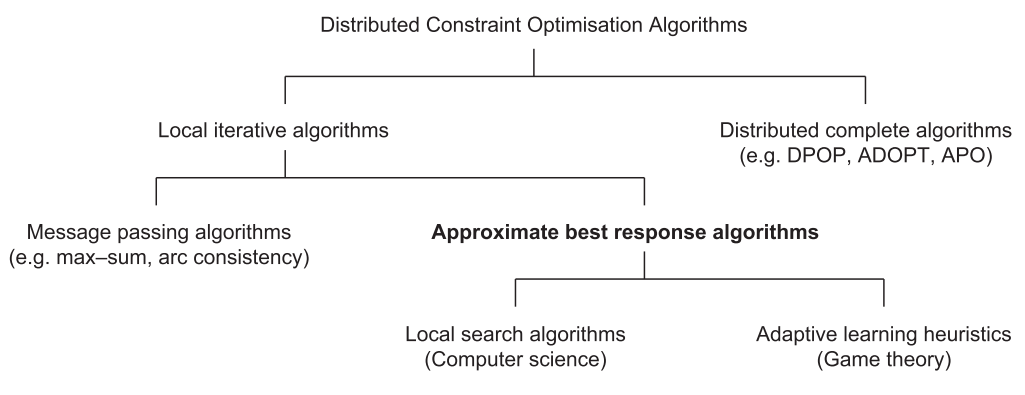
\includegraphics[width=400px]{graphics/overview_algos}
\caption{Categorization of DCO algorithms \cite{Chapman2011}}
\label{fig:categorization}
\end{figure}

Chapman et al. categorize distributed constraint optimization algorithms into local iterative and distributed complete algorithms. They further divide local iterative into message passing algorithms and approximate best response algorithms (Figure \ref{fig:categorization}). The following subsections are going to explain the differences between the three categories and introduce the concrete algorithms from these three different approaches that have been chosen for benchmarking. Advantages, as well as disadvantages will be described and which behaviour one can expect of these algorithms under certain parameters.

%Other Approaches: Bee Hive optimization, Genetic Algorithms, .. DynDCOAA, SBDO, Bee Colony algorithm, Ant colony algorithm, adopt, dsa-a, dsa-b stochastic ...\cite{Likhachev}
    
\subsection{Distributed Complete}

%-----------------  Basic Concept and Advantages Disadvantes ----------------------
Distributed complete algorithms always discover a configuration of value assignments to variables that maximizes the global utility function. This completness guarantee increases the complexity of computation and leads to exponentially growing message numbers or calculations when increasing the amount of variables in a problem. Messages between agents contain often complex structures and constraint problems usually need to be transformed to a extensive graph structure \cite{Chapman2011}. These types of algorithms therefore are not expected to scale well and quickly find qualitative solutions, but they fit well if one wants to find the maximal utility of a problem. 
    %----------------- Chosen algorithm ----------------------
\begin{figure}[H]
\centering
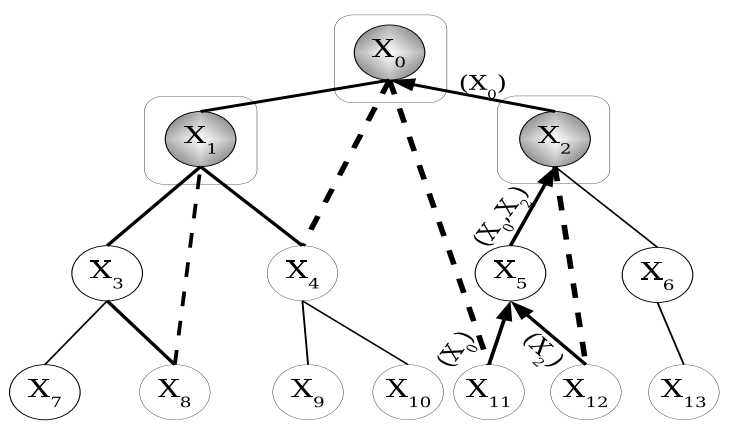
\includegraphics[width=250px]{graphics/pseudotree}
\caption{Pseudotree for DPOP \cite{Petcu2003}}
\label{fig:pseudotree}
\end{figure}

For this thesis, it was decided to implement the Dynamic Programming OPptimization algorithm (DPOP) proposed by \cite{Petcu2003} as a comparison to the local-iterative approaches. In this algorithm, constraint optimization problems need to be converted to a pseudotree (Fig. \ref{fig:pseudotree}), which is an modification of a DFS Tree. The original DCOP graph is transformed in a way that previous neighbours are placed in the same branches of a binary tree. They are connected trough ordinary tree edges, but additionaly back-edges between unconnected previous neighbours are established. The leaf nodes propose UTIL messages with their utility values for each value assignment upwards the tree and the Root node sends a VALUE message downwards containing the best value to chose. Nodes in the middle of the tree propagate UTIL and VALUE messages. The message structure is fairly complex as it involves all the pseudoparents from the back-edges and their context to a hypercube, which increases the message size exponentially. The number of messages on the other hand is linear. Through the integration of contextual values, privacy is not guaranteed in this setting.

%----------- Dynamics -----------------------
\subsection{Local-Iterative - Best Response}

%-----------------  Basic Concept and Advantages Disadvantes ----------------------
In a local-iterative best-response algorithm, agents only communicate their current state, e.g. their value assignment and react to these value messages in the best possible way from their perspective. The agents are only connected to their neighbours with whom they share constraints and there is no complex graph structure controlling the message flow \cite{Chapman2011}. Through this local property, the types of algorithms should be inherently scalable as the messages and computations do not increase exponentially. Further, this approach is optimal from a privacy perspective as the neighbours only share their current preference and no other details of their schedule. %\cite{Chapman2010} %\cite{Maheswaran} % Achtung muss das richtig paper finden
\newline\newline
%----------------- Chosen algorithm: Structure, Messages --------------------- 
For this thesis, it was decided to implement the Maximum-Gain Messaging algorithm (MGM) proposed by \cite{Yokoo1996}. In this algorithm, agents  calculate the maximal gain in utility they can achieve when assigning to another value and send this value as a message. If of all messages they received, they have the highest gain, the value is changed. Otherwise the local value stays the same. This algorithm fullfills the anytime property, i.e it can provide a solution at every timepoint during calculation and also reaches good solutions quickly \cite{Chapman2010}. As the decision of an agent depends on a complete set of message of all it's neighbours, this algorithm will supposedly not perform well in asynchronous running mode. This type of algorithm does further not always converge and does not always provide the optimal solution to a problem.

\subsection{Local-Iterative - Message Passing}
%-----------------  Basic Concept and Advantages Disadvantes ----------------------
The difference of message-passing to best-response algorithms is that the agents send and receive messages containing a specific data structure, which contains the utilities respectively costs that various assignments hold for a local variable. Received messages are used to calculate the next message that is sent to the connected neighbours. These types of algorithms are like best-response algorithms able to provide an acceptable solution in a short period of time, but also share the charasteric to sometimes not converge or not providing an optimal solution \cite{Chapman2011}.
%-----------------  Choosen algorithm ----------------------
\begin{figure}[H]
\centering
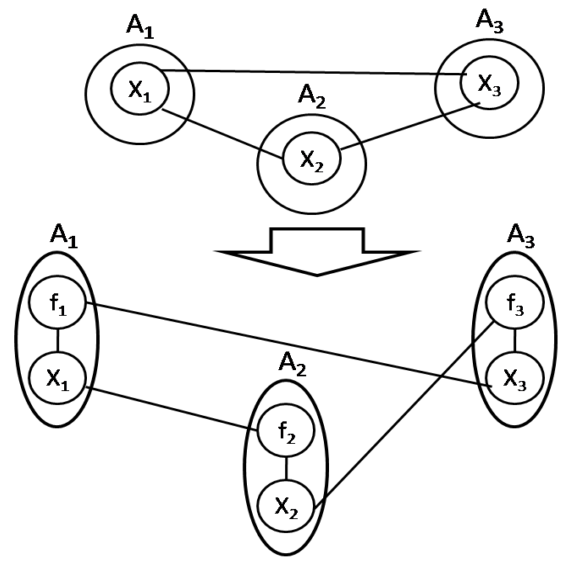
\includegraphics[width=170px]{graphics/factorgraph}
\caption{Conversion of a general DCOP to a factor graph\cite{Zivan2012}}
\label{fig:factorgraph}
\end{figure}

For this thesis, it was decided to implement the MaxSum algorithm introduced by \cite{Farinelli2008}. The algorithm has currently gotten a lot of attention from researchers. For this work, the algorithm is especially interesting because of it's proposed abilities in at least synchronously run dynamic environments.  \cite{Farinelli2008} wrote in their paper:
\begin{quote}
[...] we note that if messages are continuously propagated,
and the states of the agents are continuously updated, then the algorithm may be applied to dynamic problems where the interactions between agents, or the utilities resulting from these interactions, may change at any time.
\end{quote}

In MaxSum the original DCOP graph is transformed to a factor, which is a form of a bipartite graph and of cyclic nature (Fig. \ref{fig:factorgraph}. An agent contains after the transformation of a variable and a function node, whereas variables are connected to all corresponding function nodes of  their previous neighbours. The function nodes are vice versa connected to all previous neighbours of it's variable node. 
% ------------- Messages sent --------------------
The messages sent from variable nodes differ from the function nodes. A message from variable to function contains for every value \(d \in D_{x}\) the sum of utilities regarding this value, which the node has received from all connected function nodes. It is important to note that this sum does not include the values provided by the message target. The values are normalized at this point to avoid steadily to infinity increasing sums. A message from a function node to a variable node holds for every value  \(d \in D_{x}\)  the summation of all costs received from all connected variable nodes except the message receiver and the original cost of the constraint represented by the function node \cite{Zivan2012}.


    
    